\documentclass[a4paper,12pt]{article}

% Настройка кодировок и шрифтов
\usepackage[utf8]{inputenc}
\usepackage[russian]{babel}

\usepackage{graphicx}
\usepackage{fontspec}
\usepackage[T2A]{fontenc}
\setmainfont{Liberation Serif}

% Математические пакеты
\usepackage{amsmath, amsfonts, amssymb, amsthm}
\usepackage{geometry}
\geometry{left=20mm, right=20mm, top=20mm, bottom=20mm}

% Пакет для комплексных чисел (подчеркивание)
\newcommand{\complex}[1]{\underline{#1}}

\begin{document}

\begin{flushleft}
    Домашнее задание №2 \\
    Пахомов Владимир Юрьевич 467036
\end{flushleft}


% --- Содержание отчета ---
\section{Условие (Вариант 22)}
\begin{itemize}
    \item Методом комплексных амплитуд рассчитать мгновенные значения ЭДС источника, токов в ветвях и напряжений на элементах.
    \item Построить векторные диаграммы для любого контура и любого узла.
    \item Осуществить проверку, составив баланс мощностей.
\end{itemize}

Данные варианта:

\begin{itemize}
    \item Схема: 3.1
    \item Параметры элементов:
    \begin{itemize}
        \item $L_1 = 10 \text{ мГн} = 10 \cdot 10^{-3} \text{ Гн}$
        \item $R_2 = 7 \text{ Ом}$
        \item $C_3 = 312.5 \text{ мкФ} = 312.5 \cdot 10^{-6} \text{ Ф}$
        \item $R_4 = 7 \text{ Ом}$
        \item Элемент 5: отсутствует (принимаем провод с $Z_5 = 0$).
    \end{itemize}
    \item Заданная ЭДС: $e(t) = 30 \sin(400t) \text{ В}$.
\end{itemize}

Угловая частота: $\omega = 400 \text{ рад/с}$.

\begin{figure}[h]
    \centering
    
\includegraphics[height=9cm]{schema.png}
    \caption{Схема}
    \label{fig:schema}
\end{figure}

\section{Определение комплексных сопротивлений}
Переведем параметры элементов в комплексную форму:
\begin{enumerate}
    \item $\complex{z}_1 = j\omega L_1 = j \cdot 400 \cdot 0.01 = j4 \text{ Ом}$
    \item $\complex{z}_2 = R_2 = 7 \text{ Ом}$
    \item $\complex{z}_3 = \frac{1}{j\omega C_3} = \frac{1}{j \cdot 400 \cdot 312.5 \cdot 10^{-6}} = -j8 \text{ Ом}$
    \item $\complex{z}_4 = R_4 = 7 \text{ Ом}$
    \item $\complex{E}_m = 30 \cdot e^{j0^\circ} \text{ В}$ (комплексная амплитуда ЭДС).
\end{enumerate}

\section{Расчет токов в цепи}
Согласно схеме, цепь представляет собой последовательное соединение $\complex{z}_1$, параллельного участка ($\complex{z}_3 || \complex{z}_4$) и $\complex{z}_2$.

1. Эквивалентное сопротивление параллельного участка:
\begin{equation}
\complex{z}_{34} = \frac{\complex{z}_3 \cdot \complex{z}_4}{\complex{z}_3 + \complex{z}_4} = \frac{-j8 \cdot 7}{7 - j8} = \frac{-j56(7 + j8)}{49 + 64} = \frac{448 - j392}{113} \approx 3.965 - j3.469 \text{ Ом}
\end{equation}

2. Полное сопротивление цепи:
\begin{equation}
\complex{z}_{экв} = \complex{z}_1 + \complex{z}_{34} + \complex{z}_2 = j4 + 3.965 - j3.469 + 7 = 10.965 + j0.531 \text{ Ом}
\end{equation}
В показательной форме: $\complex{z}_{экв} \approx 10.978 \cdot e^{j2.77^\circ} \text{ Ом}$.

3. Комплексная амплитуда общего тока $i_1$:
\begin{equation}
\complex{I}_{m1} = \frac{\complex{E}_m}{\complex{z}_{экв}} = \frac{30}{10.978 \cdot e^{j2.77^\circ}} \approx 2.733 \cdot e^{-j2.77^\circ} \text{ А}
\end{equation}

4. Токи в ветвях:
\begin{equation}
\complex{I}_{m2} = \complex{I}_{m1} \frac{\complex{z}_4}{\complex{z}_3 + \complex{z}_4} = 2.733 e^{-j2.77^\circ} \frac{7}{7-j8} \approx 1.8 \cdot e^{j46.04^\circ} \text{ А}
\end{equation}
\begin{equation}
\complex{I}_{m3} = \complex{I}_{m1} \frac{\complex{z}_3}{\complex{z}_3 + \complex{z}_4} = 2.733 e^{-j2.77^\circ} \frac{-j8}{7-j8} \approx 2.057 \cdot e^{-j43.96^\circ} \text{ А}
\end{equation}

\section{Мгновенные значения}
\begin{itemize}
    \item $i_1(t) = 2.733 \sin(400t - 2.77^\circ) \text{ А}$
    \item $i_2(t) = 1.8 \sin(400t + 46.04^\circ) \text{ А}$
    \item $i_3(t) = 2.057 \sin(400t - 43.96^\circ) \text{ А}$
\end{itemize}


\section{Векторные диаграммы}

На рисунках 1 и 2 представлены векторные диаграммы, построенные по результатам расчетов. 

% Вставка диаграммы токов
\begin{figure}
    \centering
    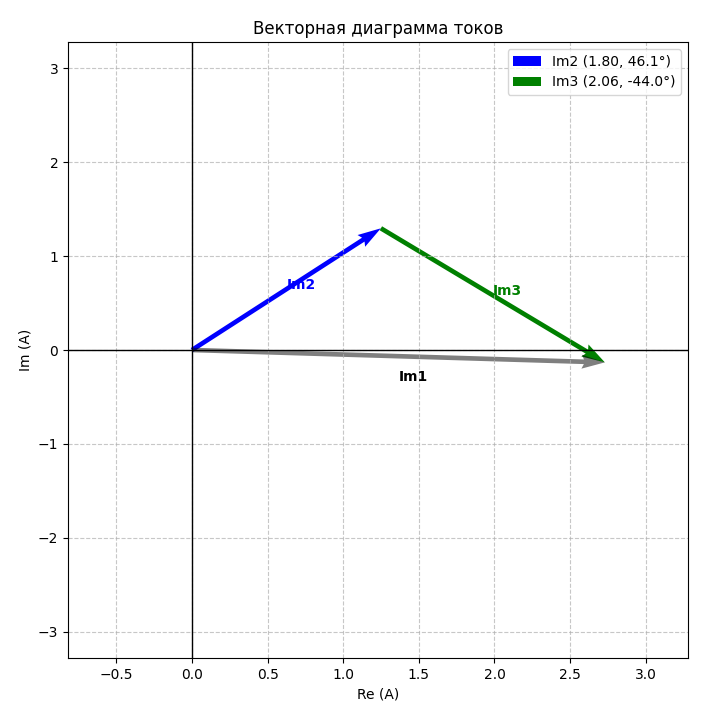
\includegraphics[height=11cm]{current.png}
    \caption{Векторная диаграмма токов (согласно ЗКI: $\complex{I}_{m1} = \complex{I}_{m2} + \complex{I}_{m3}$)}
    \label{fig:currents}
\end{figure}

% Вставка диаграммы напряжений
\begin{figure}
    \centering
    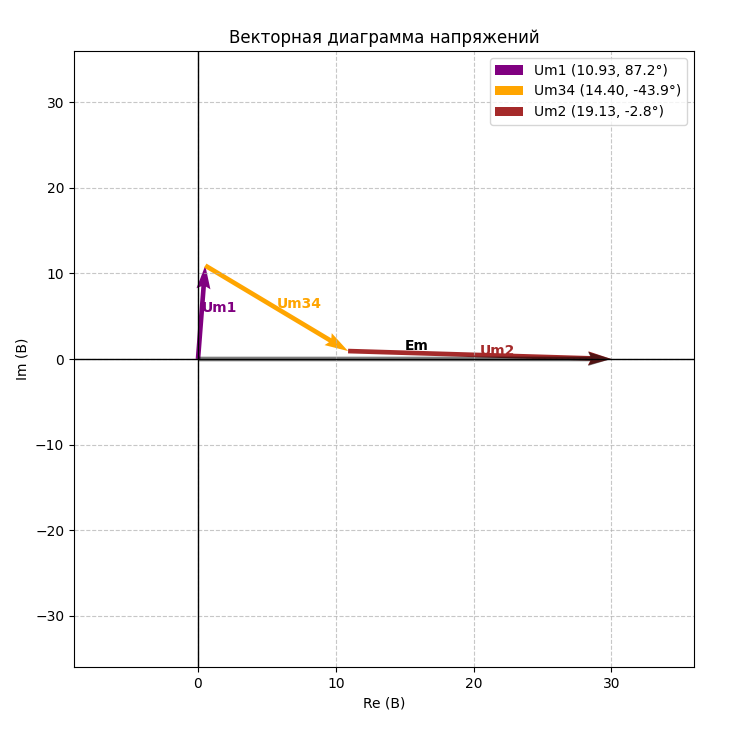
\includegraphics[height=11cm]{voltage.png}
    \caption{Векторная диаграмма напряжений (согласно ЗКII: $\complex{E}_m = \complex{U}_{m1} + \complex{U}_{m34} + \complex{U}_{m2}$)}
    \label{fig:voltages}
\end{figure}

\newpage

На диаграмме напряжений наглядно показано выполнение второго закона Кирхгофа: геометрическая сумма падений напряжений на элементах контура равна вектору ЭДС источника. На диаграмме токов показано выполнение первого закона Кирхгофа для узла.

\section{Баланс мощностей}
Комплексная мощность источника:
\begin{equation}
\complex{S}_{ист} = \frac{1}{2} \complex{E}_m \cdot \complex{I}_{m1}^* = \frac{1}{2} \cdot 30 \cdot 2.733 e^{j2.77^\circ} \approx 40.95 + j1.98 \text{ ВА}
\end{equation}

Комплексная мощность потребителей:
\begin{equation}
P = \frac{1}{2} (I_{m1}^2 R_2 + I_{m3}^2 R_4) = \frac{1}{2} (2.733^2 \cdot 7 + 2.057^2 \cdot 7) \approx 40.95 \text{ Вт}
\end{equation}
\begin{equation}
Q = \frac{1}{2} (I_{m1}^2 X_{L1} - I_{m2}^2 X_{C3}) = \frac{1}{2} (2.733^2 \cdot 4 - 1.8^2 \cdot 8) \approx 1.98 \text{ вар}
\end{equation}
$\complex{S}_{потр} = P + jQ = 40.95 + j1.98 \text{ ВА}$.
Баланс сошелся.


\end{document}